\documentclass[10pt,journal,compsoc]{IEEEtran}

\usepackage[pdftex]{graphicx}    
\usepackage{cite}
\hyphenation{op-tical net-works semi-conduc-tor}

\usepackage{listings}
\usepackage{color}

\definecolor{dkgreen}{rgb}{0,0.6,0}
\definecolor{gray}{rgb}{0.5,0.5,0.5}
\definecolor{mauve}{rgb}{0.58,0,0.82}

\lstset{frame=tb,
  language=Java,
  aboveskip=3mm,
  belowskip=3mm,
  showstringspaces=false,
  columns=flexible,
  basicstyle={\small\ttfamily},
  numbers=none,
  numberstyle=\tiny\color{gray},
  keywordstyle=\color{blue},
  commentstyle=\color{dkgreen},
  stringstyle=\color{mauve},
  breaklines=true,
  breakatwhitespace=true,
  tabsize=3
}

\begin{document}

\title{Training a Robotic Arm using Deep Q-Network}

\author{Peng Xu}

\markboth{Deep RL project, Robotic Nanodegree, Udacity}%
{}
\IEEEtitleabstractindextext{%

\begin{abstract}
A Deep Q-Network is used to train a 2 degree Robotic Arm to grasp the tube.
\end{abstract}

% Note that keywords are not normally used for peerreview papers.
\begin{IEEEkeywords}
Robotic Arm, Deep Reinforcement Learning, Deep Q-Network, Gazebo.
\end{IEEEkeywords}}


\maketitle
\IEEEdisplaynontitleabstractindextext
\IEEEpeerreviewmaketitle
\section{Introduction}
\label{sec:introduction}

\IEEEPARstart{T}{he} project goal is to create a DQN (Deep Q-Network) agent and define reward functions to teach a robotic arm to carry out two primary objectives:

\begin{itemize}
    \item Have any part of the robot arm touch the object of interest, with at least a 90\% accuracy.
    \item Have only the gripper base of the robot arm touch the object, with at least a 80\% accuracy.
\end{itemize}

Reinforcement Learning is a type of machine learning that allows you to create AI agents that learn from the environment by interacting with it. Just like how we learn to ride a bicycle, this kind of AI learns by trial and error. As seen in Fig. \ref{fig:rl-interact}, the robot represents the AI agent, which acts on the environment. After each action, the agent receives the feedback. The feedback consists of the reward and next state of the environment. The reward is usually defined by a human. If we use the analogy of the bicycle, we can define reward as the distance from the original starting point.

With algorithms such as DQN, one can learn by choosing the actions and observing their results directly in the environment.

%example for inserting image
\begin{figure}[thpb]
      \centering
      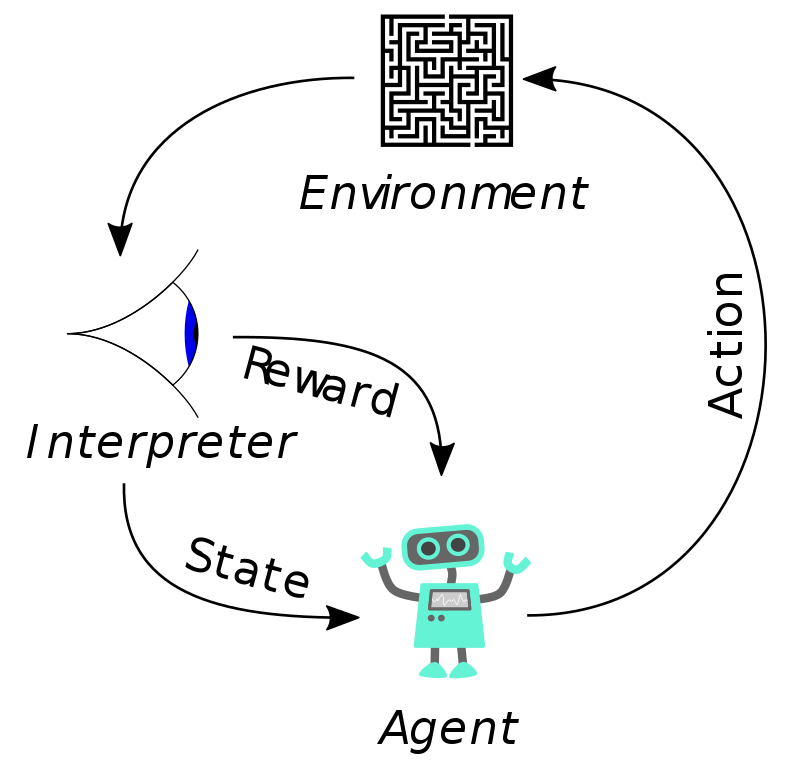
\includegraphics[width=\linewidth]{figs/Reinforcement_learning_diagram.png}
      \caption{How an agent interacts with the environment.}
      \label{fig:rl-interact}
\end{figure}

\section{Formulation}

\subsection{Reward Functions}

The reward function is a crucial component in guiding the DQN agent through the process of learning to manipulate the arm. After every end of episode (EOE), a particular reward is issued, depending on the triggering event.

\subsubsection{Reward for Timeout}

REWARD\_LOSS is issued when the current episode exceeds 100 steps.

\subsubsection{Reward for Robot Gripper Hitting the Ground}

REWARD\_LOSS is issued when the arm contacts the ground.

Whether the arm contacts the ground is detected using the GetBoundingBox() function from the Gazebo API which provides the min/max XYZ values of the arm. Collisions can be thought to happen when the Z value of the ground is below the one of the arm.

\begin{lstlisting}
bool checkGroundContact = (gripBBox.max.z <= groundContact) && (gripBBox.min.z <= groundContact);

if(checkGroundContact)
{

  if(DEBUG){printf("GROUND CONTACT, EOE\n");}

  rewardHistory = REWARD_LOSS;
  newReward     = true;
  endEpisode    = true;
}
\end{lstlisting}

\subsubsection{Issue an interim reward based on the distance to the object}

In most steps, the robot arm cannot end the current episode by the desired contact. But it should be always either moving closer or further to the goal. An interim reward function was in this concept implemented by measuring how far away from the desired contact position which would help guide the arm towards the object and reduce the training time. The reward is proportional to the change in distance between the arm and the object. If the arm is moving away from the object, the interim reward will be negative. Else, the interim reward will be positive. The raw values cause the arm to have a jerking movement, so they are smoothed by taking a moving average. Finally, due to the agent's tendency to remain still, a time penalty was introduced to encourage the agent to finish as quickly as possible.

\begin{lstlisting}
const float distGoal = BoxDistance(propBBox, gripBBox); // compute the reward from distance to the goal

if(DEBUG){printf("distance('%s', '%s') = %f\n", gripper->GetName().c_str(), prop->model->GetName().c_str(), distGoal);}

if( episodeFrames > 1 )
{
const float distDelta  = lastGoalDistance - distGoal;

// compute the smoothed moving average of the delta of the distance to the goal
avgGoalDelta  = (avgGoalDelta * ALPHA) + (distDelta * (1.0f - ALPHA));

if(avgGoalDelta > 0)
  rewardHistory = REWARD_WIN;
else
  rewardHistory = REWARD_LOSS * distGoal;

// we want to be moving
if (abs(avgGoalDelta) < .001f)
  rewardHistory += REWARD_LOSS;

newReward     = true;
}

lastGoalDistance = distGoal;
\end{lstlisting}

\subsubsection{Issue a reward based on collision between the arm and the object}

REWARD\_WIN is issued when any part of the arm contacts the object in Task 1 or when only the gripper base contacts the object in Task 2.

For task 1:

\begin{lstlisting}
bool collisionCheckArm = 
(strcmp(contacts->contact(i).collision1()
.c_str(), COLLISION_ITEM) == 0);
\end{lstlisting}

For task 2:

\begin{lstlisting}
bool collisionCheckArm = 
(strcmp(contacts->contact(i).collision1()
.c_str(), COLLISION_ITEM) == 0) && 
(strcmp(contacts->contact(i).collision2()
.c_str(), COLLISION_POINT) == 0);
\end{lstlisting}

If the disired contact is detected, a positive reward, REWARD\_WIN, would be issued and end the current episode. Else, a small punishment or a negative reward should be assigned to the reward function for the time consuming.

\begin{lstlisting}
if (collisionCheckArm)
{
  rewardHistory = REWARD_WIN;
  newReward  = true;
  endEpisode = true;
  return;
} else {
  rewardHistory = REWARD_LOSS * 0.1f;
  newReward  = true;
  endEpisode = false;
}
\end{lstlisting}

\subsection{Hyperparameters}

In Q-Learning, epsilon-Greedy is a typical exploration method used to encourage an agent to explore more of the state-action space. The larger the value, the more frequently a random action is chosen instead of one with the highest q-value. EPS\_START defines the initial value. 0.9f ensures the agent is exposed to many state-action spaces. EPS\_END defines the final value. 0.0f ensures that only learned actions with the highest q-value is used once it has been sufficiently exposed. EPS\_DECAY defines the rate by which the value decays from initial to final over time. 

\begin{lstlisting}
// Define DQN API Settings

#define INPUT_CHANNELS 3
#define ALLOW_RANDOM true
#define DEBUG_DQN false
#define GAMMA 0.9f
#define EPS_START 0.9f
#define EPS_END 0.05f
#define EPS_DECAY 200
\end{lstlisting}

The input dimensions were set to match that of the image captured by the camera: 64 x 64 pixels. "Adam" was adopted as the optimizer. LSTM was set to true to enable the agent to consider previously encountered states. LSTM\_SIZE was set to 256 as default, strengthening the agent's ability to consider more complex moves. A LEARNING\_RATE of 0.1f was sufficient for Task 1, but not for Task 2 as it took much too long learn. For better ensurance of convergence, the value was decreased to 0.01f. The BATCH\_SIZE was decreased from 64 to 32 considering the computing power.

\begin{lstlisting}
#define INPUT_WIDTH   64
#define INPUT_HEIGHT  64
#define OPTIMIZER "Adam"
#define LEARNING_RATE 0.01f
#define REPLAY_MEMORY 10000
#define BATCH_SIZE 32
#define USE_LSTM true
#define LSTM_SIZE 256
\end{lstlisting}

REWARD\_INTERIM was the reward incrementally issued to lead the agent towards the object. ALPHA was used to calculate a moving average of the delta distances. To deter the agent from standing still, a TIME\_PENALTY was introduced. All three of these were tuned concurrently to find the values that issued appropriate interim rewards.

\begin{lstlisting}
// Reward Parameters
#define REWARD_WIN  30.0f
#define REWARD_LOSS -30.0f
#define REWARD_INTERIM 5.0f
#define ALPHA 0.6f
#define TIME_PENALTY 0.4f
\end{lstlisting}


\section{Results}

\subsection{Task 1: Touch Any Part of the Robot Arm}

A screen shot is shown as in Fig. \ref{fig:task1-sc}. The required accuracy 90\% was reached after about 220 episodes, which is quite efficient.

\begin{figure}[thpb]
      \centering
      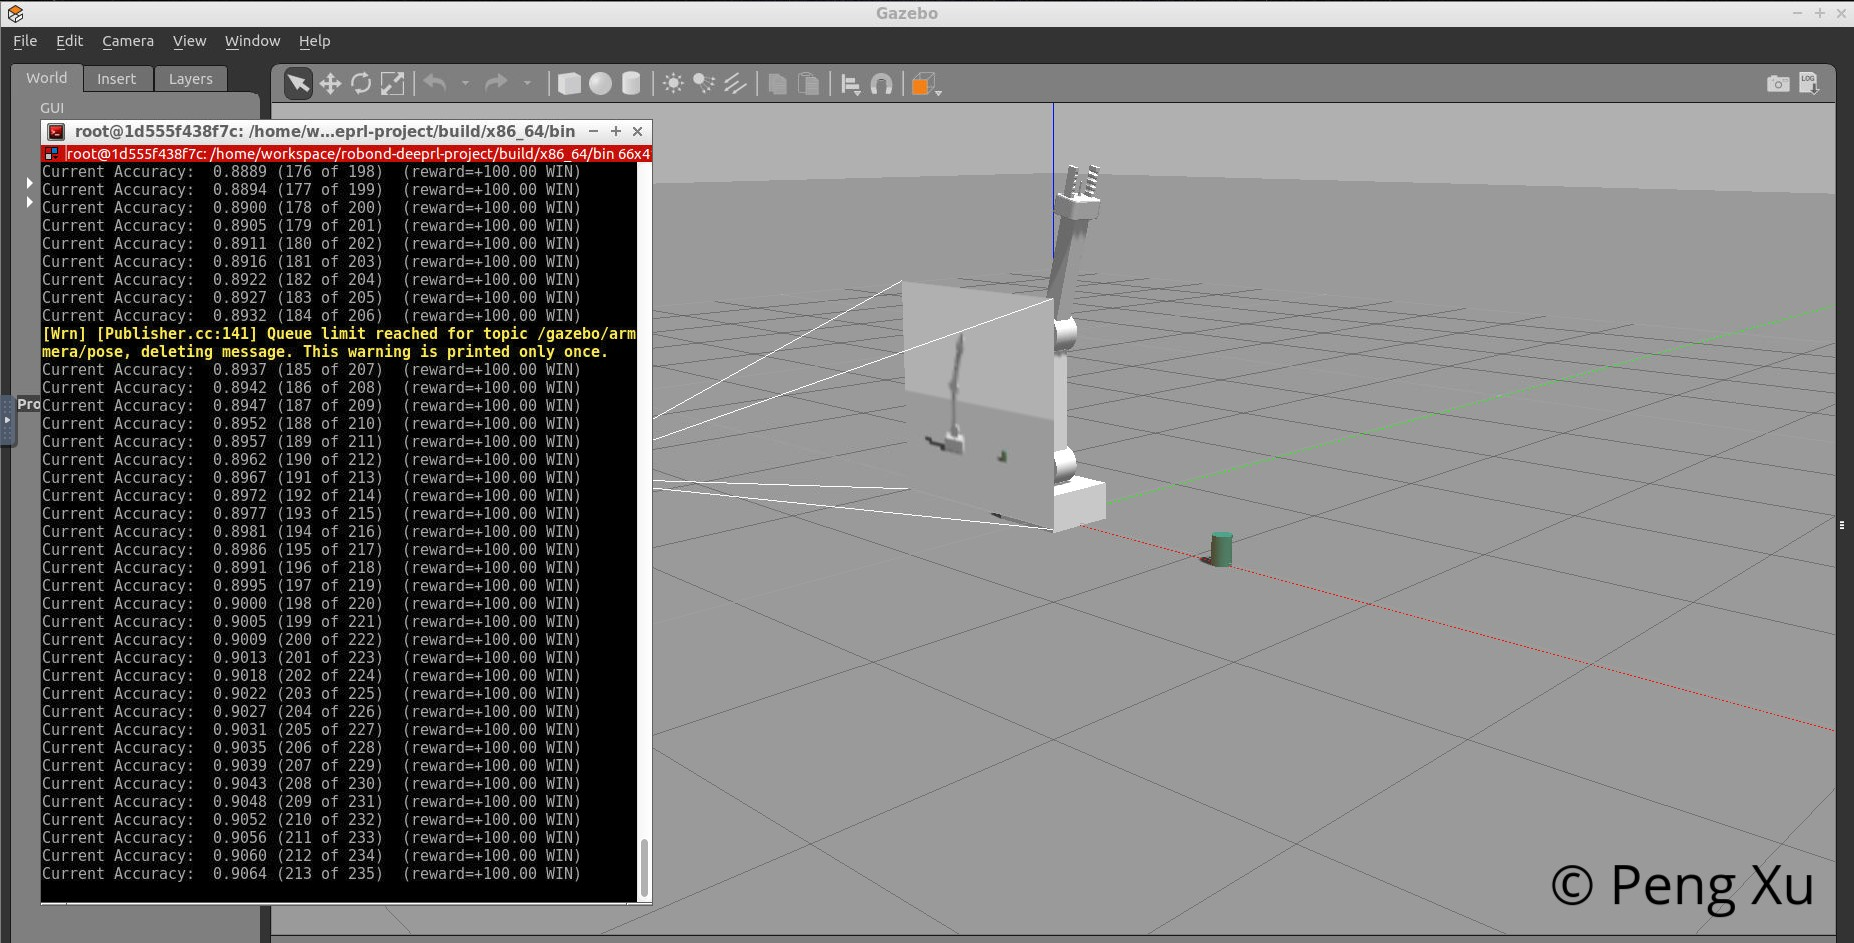
\includegraphics[width=\linewidth]{figs/task1-sc.png}
      \caption{Task 1: Touch Any Part of the Robot Arm.}
      \label{fig:task1-sc}
\end{figure}

\subsection{Task 2: Touch the Gripper Base of the Robot Arm}

A screen shot is shown as in Fig. \ref{fig:task2-sc}. The required accuracy 80\% was reached after around 1000 episodes. 

\begin{figure}[thpb]
      \centering
      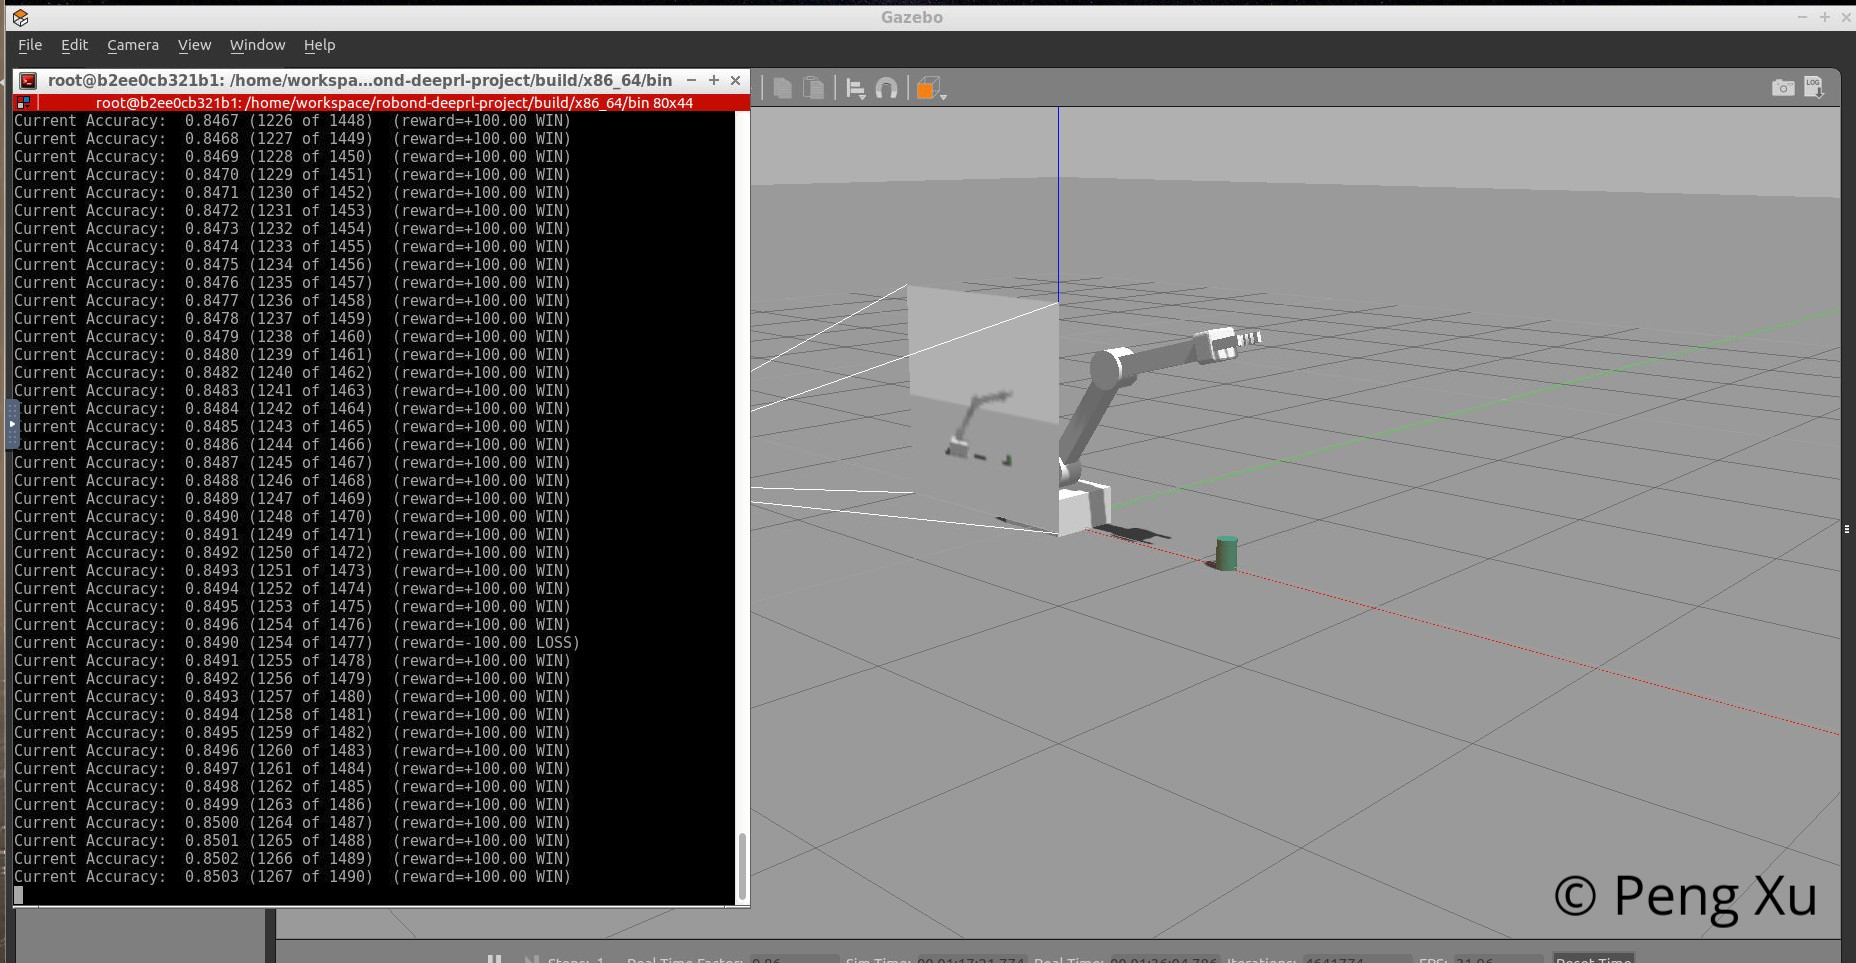
\includegraphics[width=\linewidth]{figs/task2-sc.png}
      \caption{Task 2: Touch the Gripper Base of the Robot Arm.}
      \label{fig:task2-sc}
\end{figure}

\section{Discussion}

The DQN was able to successfully complete both tasks. Task 1 parameters were consistent in results of 90\% within the range of 250 episodes. Task 2 parameters were less consistent which due to the higher requirement of the reward functions. The beginning stage significantly influenced the convergence time. If the beginning episodes happen to perform well it would be more likely to reach the success rate in a shorter time.

\section{Future work}

Deep Reinforcement Learning methods are promising on training robots. There are several aspects that can be dived deeper, such as

\begin{itemize}
    \item High dimensional motion control.
    \item Other more efficient Deep Reinforcement Learning methods.
    \item More realistic simulation environments prepared for transfer learning.
\end{itemize}

Those above experiments relys on heavy computation ability namely power GPUs and careful hyper-parameter tuning.


\end{document}